\documentclass[12pt,letterpaper]{article}
\usepackage[margin=1in]{geometry}
\usepackage{mathptmx}
\usepackage{amsmath}
\usepackage{graphicx}
\usepackage{booktabs}
\usepackage{xcolor}
\usepackage{siunitx}
\usepackage{tikz}
\usetikzlibrary{positioning}
\usepackage[hidelinks]{hyperref}
\usepackage[numbers]{natbib}
\usepackage[font=small,skip=3pt]{caption}
\usepackage{titlesec}
\titleformat{\section}{\centering\normalsize\bfseries}{\thesection.}{0.5em}{\MakeUppercase}
\titleformat{\subsection}{\normalsize\bfseries}{\thesubsection}{0.5em}{}
\titlespacing*{\section}{0pt}{2\baselineskip}{\baselineskip}
\titlespacing*{\subsection}{0pt}{\baselineskip}{0.5\baselineskip}
\usepackage{enumitem}
\setlist{nosep,leftmargin=3em,topsep=\baselineskip}
\setlength{\parindent}{0pt}
\setlength{\emergencystretch}{1.2em}
\setlength{\parskip}{\baselineskip}
\renewcommand{\topfraction}{0.95}
\renewcommand{\bottomfraction}{0.9}
\renewcommand{\textfraction}{0.05}
\renewcommand{\floatpagefraction}{0.85}
\setlength{\textfloatsep}{10pt plus 2pt minus 2pt}
\setlength{\intextsep}{10pt plus 2pt minus 2pt}

% Items the authors must confirm before submission render in red. Define
% \needsverify as \@gobble (or an empty macro) for the camera-ready copy.
\newcommand{\needsverify}[1]{\textcolor{red}{[Verify: #1]}}

\title{}
\date{}

\begin{document}

\begin{center}
{\fontsize{16}{19}\selectfont\bfseries CLOSING THE CONFIGURATION CONSISTENCY GAP IN A
COTS IRIG-106 PCM TELEMETRY SYSTEM: VERIFICATION, IDENTIFICATION, AND AUTHENTICATION IN
THE BITSTREAM\par}
\vspace{2\baselineskip}
{\fontsize{14}{17}\selectfont\bfseries Chiekeziem Udenta, Mason Joyner,
Dominique Stewart\par}
\vspace{0.6\baselineskip}
{\fontsize{14}{17}\selectfont\bfseries Student Paper Advisor: Dr.\ Oluwatobi Busari\par}
{\fontsize{12}{14}\selectfont\bfseries Morgan State University, Baltimore, MD
\\ Rochester Institute of Technology, Rochester, NY\par}
\vspace{4\baselineskip}
\end{center}

\begin{abstract}
This paper describes the design, configuration, and staged verification of an IRIG-106
Chapter~4 PCM telemetry system for a student-built liquid-propellant rocket: a
twelve-sensor suite acquired through a Curtiss-Wright KAM-500 chassis, an S-band PCM/FM
downlink at 3.2768~Mb/s, and a Lumistar LS-28 ground segment. We argue that in a modern
COTS telemetry system the dominant integration risk has migrated from hardware to
\emph{deployment consistency} between the frame definition compiled into the chassis and
the parameter database loaded on the ground, a gap that neither receiver lock, frame
synchronization, nor the toolchain's structural validation can see. We demonstrate the
failure mode live and show that a single frame-embedded counter word exposes it on the
first frame, with zero false passes over 111~s under a three-frame window. Link
characterization to 120.6~dB equivalent path loss recorded zero bit errors;
temperature channels were verified at the ice point to a mean error of 0.26~\si{\celsius}
or better through the complete chain; all four pressure channels collapse to a uniform
0.008\%-of-full-scale noise floor; and the onboard recorder supplied every one of 854
frames lost during a 13.4~s transmitter outage, 99.6\% sample-exact against the downlink.
We then extend the argument from consistency to \emph{identity} and \emph{authenticity}:
a configuration hash identifies the frame map by content rather than by version number,
and a lightweight authenticated-encryption layer, implementable between the PCM encoder
and the transmitter without any change to the PCM/FM waveform, receiver, or decommutator,
reuses the same counter word as its nonce. In software demonstration the layer rejects
every injected and replayed frame, resumes on the first frame after outages that span a
counter wrap, and costs 2--6\% of the frame. Configuration consistency, we conclude, is a
property to be verified, identified, and authenticated in the bitstream, not assumed from
the toolchain.
\end{abstract}

\noindent\textbf{Key Words:} PCM telemetry; IRIG-106; configuration management;
verification; authenticated encryption; sounding rocket

\section{Introduction}

Morgan State University's Rocket Propulsion Laboratory is developing a liquid-propellant
(RP-1/LOX) sounding rocket with a design apogee of 50{,}000~ft (15.2~km). The vehicle
carries two video channels, four pressure transducers spanning 350 to 5000~psi, three
thermocouples, a barometric altimeter, and a GNSS receiver chosen specifically because it
continues to report beyond civilian-receiver velocity and altitude thresholds. Live
visualization of that data during the flight is a program requirement, and the data volume
rules out the low-rate links common in student avionics. Telemetry links trade data rate
against robustness: ISRO's Pisharoty radiosonde pairs low-rate FSK with Reed--Solomon
coding~\cite{divya2014}, and NPS's Adamos avionics bay uses a 915~MHz LoRa transceiver,
trading standards compliance for cost~\cite{adamos2021}. This system occupies a third
point, an IRIG-106 Chapter~4 PCM stream~\cite{irig106} over S-band PCM/FM, because the
data exceed what low-throughput links carry and because the standard provides
interoperability with established range equipment.

Standards compliance does not eliminate integration risk; it relocates it. Four decades of
hand-built PCM encoders realized frame structures in programmable logic and were verified
at the level of wiring~\cite{rochefort1991,salib2024}. In a COTS implementation the frame
definition is compiled in a vendor environment, and the risk moves to \emph{deployment}:
one compile yields a chassis programming action and a ground file pair, performed
separately, and the two must agree exactly or an error propagates through an entire dataset
as plausible but wrong engineering values. In the worst documented case, recovering a
mismatched Chapter~4 recording required manual, hex-level reconstruction~\cite{rettig2017}.

The standard itself offers partial remedies, and it is important to say precisely what
they do and do not cover. The Telemetry Attributes Transfer Standard (TMATS, IRIG 106
Chapter~9, with its handbook RCC~124~\cite{rcc124}) is a vendor-neutral description of the
PCM format intended to move from the instrumentation side to the ground side; it collapses
a file \emph{pair} to a single file where both toolchains support it, but it is still a
file, and it says nothing about whether the configuration \emph{running} in the chassis is
the one described. Chapter~10/11 recording embeds the TMATS in the recording's setup
record, which binds a \emph{recording} to its configuration. Chapter~7 packet telemetry
carries Chapter~11 packets inside a Chapter~4 frame~\cite{hoffman2019}, which would make
the downlink and the onboard record the same data format and dissolve the record-merge
problem of \S\ref{sec:res-reacq}. None of these verifies, at the moment of reception, that
the ground's belief about the frame matches what the vehicle is transmitting. That
verification can only travel in the bitstream, the one channel that physically connects
the two deployments, and this paper treats it as the system's central engineering problem.

Ground-side reception carries its own trade-offs: larger ranges combat fades with multiple
separated antennas recombined by best-source selection~\cite{bastie2022} or by digitizing
at the antenna into all-digital multi-channel receivers~\cite{bastie2024}. A single
dual-channel receiver suffices for one test article, but our two-channel data
(\S\ref{sec:res-link}) already exhibit the decorrelated fading that motivates source
selection at range scale.

The paper makes four contributions.
\begin{enumerate}
  \item A staged, pre-declared verification campaign for a COTS Chapter~4 system (link,
  sensor chain, configuration fault injection, dropout and recovery), with results through
  the complete acquisition--transmission--decommutation chain.
  \item A live demonstration of air/ground configuration skew that leaves receiver lock
  and SFID cycling intact, and of its detection on the first frame by a chassis-native
  counter word, at 1\% of link capacity.
  \item An extension from \emph{consistency} to \emph{identity}: a configuration hash
  transmitted alongside the counter identifies the frame map by content, so that a
  mismatch names the differing configuration rather than merely signalling one.
  \item An extension from identity to \emph{authenticity}: a lightweight
  authenticated-encryption layer that fits entirely inside the existing PCM/FM hardware
  envelope, reuses the counter word as its nonce, and is demonstrated in software against
  injection, replay, dropout, and skew.
\end{enumerate}

Section~\ref{sec:architecture} describes the architecture, Section~\ref{sec:frame} the
frame design including the reserved security words, Section~\ref{sec:methodology} the
verification methodology and the security layer, Section~\ref{sec:results} the results,
and Section~\ref{sec:lessons} the lessons learned.

\section{System Architecture}\label{sec:architecture}

\subsection{Sensor Suite and Acquisition Mapping}\label{sec:sensors}

\begin{table}[htbp]
  \centering
  \caption{Sensor suite and acquisition mapping.}
  \label{tab:sensors}
  \footnotesize
  \begin{tabular}{@{}p{3.4cm}cp{4.8cm}p{4.6cm}@{}}
    \toprule
    Sensor & Qty & Measurement & Acquisition card \\
    \midrule
    RV-CAM HD19 & 2 & Video (H.264 encoded) & 2$\times$ KAD/VID/106 \\
    UNIK 5000 & 4 & Pressure: 350/700/1000/5000 psi FS & KAD/ADC/134 \\
    Omega KMQSS-062U-6 & 3 & Temperature (type K) & KAD/TDC/102 \\
    Trans Cal SSD120(XX)N & 1 & Barometric altitude, RS-232 & KAD/UBM/105 \\
    NovaTel PwrPak7 & 1 & GNSS position/velocity/time & KAM/TCG/105 (+UBM/105) \\
    Multitronix Mx210 & 1 & Recovery altimeter & Independent RF link (own TX/ground RX) \\
    \bottomrule
  \end{tabular}
\end{table}

Three integration decisions merit discussion. First, the PwrPak7 is an \emph{external}
GNSS receiver: civilian receivers cease reporting beyond the legacy CoCom thresholds
(${\approx}$515~m/s and 18~km, carried forward in the Wassenaar list and ITAR
Category~XV~\cite{wassenaar,itar}), whereas the PwrPak7 measures continuously to at least
711~m/s and supports a higher output rate than the TCG/105's onboard receiver. Second, GNSS
serial data is routed through the KAD/UBM/105 in addition to the TCG/105, raising the
position/velocity update rate from 1 to 10~Hz. Third, the recovery altimeter that commands
parachute deployment is kept entirely outside the telemetry chain, on its own transmitter
and ground receiver, so that no failure of the data link, and no key-management or
configuration failure introduced by the mechanisms of this paper, can touch a
safety-of-flight function.

The system architecture is shown in Figure~\ref{fig:architecture}. All acquisition cards
reside in a KAM/CHS/13U chassis; a KAD/BCU/101 serves as backplane controller and IRIG-106
Chapter~4 PCM encoder, and a KAM/MEM/113 logs the full acquired stream to CompactFlash as a
recovery record independent of the RF downlink.

\begin{figure}[htbp]
  \centering
  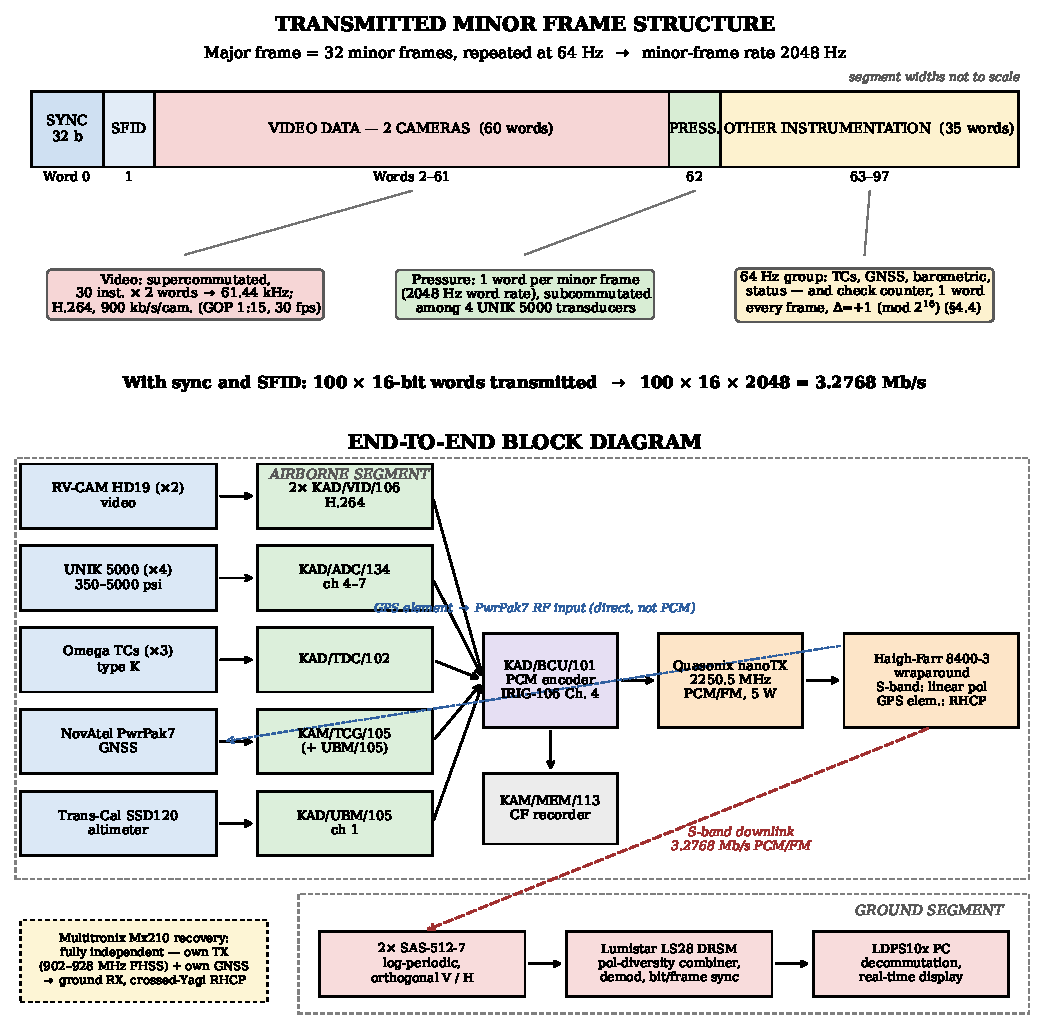
\includegraphics[width=0.94\textwidth]{figs/fig_system_overview.pdf}
  \caption{End-to-end telemetry system: transmitted minor-frame structure and parameter
  allocation (top), and hardware block diagram from sensors through PCM encoding, RF
  transmission, and ground decommutation (bottom). \needsverify{redraw the top panel with
  the 16-bit word indexing of \S\ref{sec:frame}: 100 words, sync = words 0--1, SFID =
  word 2, and the reserved security words}.}
  \label{fig:architecture}
\end{figure}

\subsection{RF Link}\label{sec:rf}

The BCU/101 outputs a baseband PCM clock-and-data stream (NRZ-L) that drives a Quasonix
nanoTX transmitter (2200.5--2394.5~MHz, 5~W, heat-sink mounted), configured at 2250.5~MHz
with PCM/FM at 3.2768~Mb/s. The modulation is a property of the transmitter, not the
chassis: the nanoTX family is multi-waveform and offers an LDPC forward-error-correction
option whose flight-test gains are documented~\cite{temple2021} and whose rate-compatible,
bandwidth-efficient successors are an active research area~\cite{cummins2024}, and we record here the state of the loaned unit so that the
choice of PCM/FM is a documented decision rather than an assumed constraint.
\needsverify{state whether the loaned nanoTX carries the SOQPSK-TG and LDPC options; if
so, give one sentence each on why they were not enabled for this flight (receiver option
set, bandwidth authorization, schedule)}. PCM/FM at 3.2768~Mb/s occupies approximately
3.8~MHz (99\% bandwidth, premodulation-filtered), within the 2200--2290~MHz band under
\needsverify{frequency authorization: cite the coordination path and assignment}.

The output feeds a Haigh-Farr 7-inch wraparound antenna (P/N~8400-3) whose S-band element
radiates the downlink; a separate RHCP element receives GPS for the PwrPak7. Calibrated
cuts of the flight unit (S/N~0876, at 2.21, 2.2525, and 2.295~GHz) establish that the
S-band element is \emph{linearly} polarized, ${\approx}$0 to $+5$~dBi over broad sectors
with $-25$ to $-30$~dB cut-plane nulls (pattern data on file). The link budget of
\S\ref{sec:linkbudget} uses the conservative $-1$~dBi figure. Vehicle roll rotates the
transmitted polarization relative to any fixed ground aperture, with consequences
addressed in \S\ref{sec:ground}. The stream is dominated by video (60 of 100 transmitted
words).

\subsection{Ground Segment}\label{sec:ground}

The ground station is a Lumistar LS-28 DRSM, a dual-channel receiver performing
demodulation, bit synchronization, and onboard IRIG-106 frame synchronization and
decommutation, feeding a PC where the LDPS10x suite maps the stream to engineering
parameters using a hardware interface file and parameter database exported from DAS
Studio; frame lock is keyed to the sync word, with the SFID tracking subcommutation pages.
The LS-28 also emits each decommutated minor frame as a TMoIP packet, which is the point at
which the ground software of \S\ref{sec:security} operates.

The flight ground antennas are the SAS-512-7 log-periodic antennas used throughout the test
campaign, with receive antenna gain identified as the primary area for future improvement.
As directional apertures they must be pointed along the flight path; boresight tracking of
the trajectory is an operational task of the ground crew. Because the airborne S-band
element is linearly polarized and the vehicle rolls, the transmitted polarization rotates
continuously relative to a fixed linear receive aperture. A circularly polarized ground
antenna would remove the roll fade at a fixed 3~dB cost with one receive chain; we instead
mount the two log-periodics orthogonally, one vertical and one horizontal, with the
receiver in polarization-diversity combined mode (LS-28 pre-detection optimal-ratio
combiner, ${>}2.6$~dB S/N improvement near threshold), because this retains the
spatial-diversity gain against the multipath measured in \S\ref{sec:res-link}, which a
single circular aperture would not. Between orthogonal apertures roll fades are
anti-correlated by construction: linear transmission at angle $\theta$ couples as
$\cos^2\theta$ and $\sin^2\theta$ respectively, so the ideal combined response
$\propto \cos^2\theta + \sin^2\theta = 1$ is roll-invariant.

The receiver threshold is estimated from datasheet parameters, as the LS-28 specifies no
single sensitivity figure: a 3--4~dB noise figure, an IF bandwidth auto-selected to match
the 3.2768~Mb/s PCM/FM waveform (${\approx}3.3$~MHz), and a multi-symbol PCM/FM threshold
of ${\approx}9$--10~dB $E_b/N_0$ give an estimated sensitivity of ${\approx}{-95}$~dBm.
Against the 30~dB fade-margin criterion of Table~\ref{tab:matrix}, the flight condition
would require ${\approx}24$~dBi of aligned linear receive gain; the 6.5~dBi log-periodics
instead provide a predicted ${\approx}12$~dB, a documented shortfall accepted for this
flight and mitigated by diversity combining, the onboard MEM/113 record, and the independent
Mx210 link, with a higher-gain aperture (or LDPC coding, if the option set permits) as the
improvement path.

\section{Telemetry Frame Design}\label{sec:frame}

The stream is transmitted at 3.2768~Mb/s in 16-bit words. Each transmitted minor frame is
100 words: a 32-bit frame synchronization pattern occupying words~0--1, a 16-bit Subframe
Identification (SFID) word at word~2, and 97 data words. Thirty-two minor frames form a
major frame repeating at 64~Hz, so the minor-frame rate is $32 \times 64 = 2048$~s$^{-1}$
and $100 \times 16 \times 2048 = 3.2768$~Mb/s. Captured TMoIP packets corroborate this
independently: 232-byte payloads decompose as $8 + 24 + 200$~bytes, the 200 bytes being
exactly the 100 sixteen-bit transmitted words, one packet per minor frame; and the LS-28
bit-synchronizer count of $3.2766$--$3.2782 \times 10^{6}$~counts/s (\S\ref{sec:res-reacq})
confirms 1600 bits per frame. \needsverify{the earlier draft and frame-map figure described
a 98-word frame with a 16-bit sync value (0xEB90) of 32-bit length; confirm the DAS Studio
sync pattern (the IRIG 106 Appendix~C 32-bit recommendation is 0xFE6B2840) and make the
figure agree with this paragraph}.

The majority of each minor frame carries two supercommutated video channels: 30 instances
per minor frame (60 words), 15 per camera, grouped by DAS Studio~3 Burst Placement into
uniformly repeated bursts, for an effective video update rate of 61.44~kHz. The
corresponding transport allocation is 983.04~kb/s per camera, carrying the VID/106's
constant-bit-rate H.264 output (900~kb/s per camera, 30~frames/s NTSC,
\needsverify{GOP length: 15 frames gives a 0.500~s keyframe interval, 16 gives the 0.533~s
used in Table~\ref{tab:matrix}; state the configured value and use it consistently}).
One word per minor frame carries pressure data and the remaining words carry GNSS,
thermocouple, barometric, and status data at the 64~Hz major-frame rate.
\needsverify{pressure commutation: the earlier draft called the pressure word
``subcommutated among the four transducers'' (512~Hz each) yet reported 2048~Hz per
channel in \S\ref{sec:res-chan}; a subcommutated slot does not deliver the full rate to one
sensor because the others are idle. Either the test configurations placed one sensor at the
full rate (then say so, and that the flight frame differs) or the word is not
subcommutated. Delete the alternative that does not apply}.

\paragraph{Reserved security words.}
Three word positions are reserved in the DAS Studio map as spare parameters and are
overwritten downstream of the encoder by the device described in \S\ref{sec:security}:
word~3 carries the low 16 bits of a frame counter (the check word of \S\ref{sec:fault}),
word~4 carries a subcommutated \emph{security channel} (one 16-bit word per minor frame,
indexed by SFID, forming a 64-byte record per major frame), and the last two or four words
of the minor frame carry an authentication tag. Figure~\ref{fig:secframe} shows the layout.
The baseline frame, without the security device, is the same layout with the counter
supplied by the chassis-native counter parameter and the other reserved words constant.
The video, pressure, and instrumentation allocations are otherwise unchanged; the reserved
words come from the 35-word instrumentation region, which has spare capacity at 64~Hz.

\begin{figure}[htbp]
  \centering
  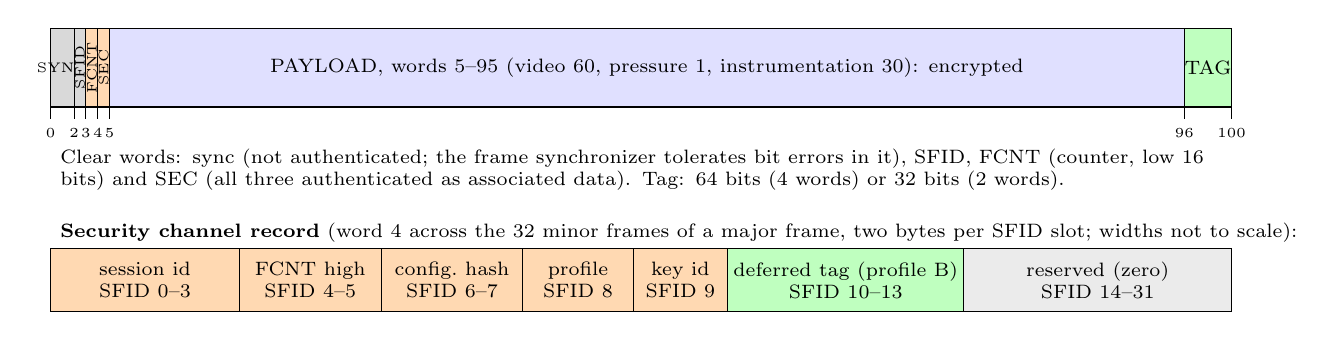
\begin{tikzpicture}[x=1mm,y=1mm,font=\scriptsize]
    % minor frame bar: 100 words -> 150 mm (to scale)
    \def\W{1.5}
    \draw[fill=black!15] (0,0) rectangle (2*\W,10);     \node at (1*\W,5) {\tiny SYNC};
    \draw[fill=black!15] (2*\W,0) rectangle (3*\W,10);  \node[rotate=90] at (2.5*\W,5) {\tiny SFID};
    \draw[fill=orange!30] (3*\W,0) rectangle (4*\W,10); \node[rotate=90] at (3.5*\W,5) {\tiny FCNT};
    \draw[fill=orange!30] (4*\W,0) rectangle (5*\W,10); \node[rotate=90] at (4.5*\W,5) {\tiny SEC};
    \draw[fill=blue!12] (5*\W,0) rectangle (96*\W,10);  \node at (50.5*\W,5) {PAYLOAD, words 5--95 (video 60, pressure 1, instrumentation 30): encrypted};
    \draw[fill=green!25] (96*\W,0) rectangle (100*\W,10); \node at (98*\W,5) {TAG};
    \foreach \x/\l in {0/0,2/2,3/3,4/4,5/5,96/96,100/100} {\draw (\x*\W,0) -- (\x*\W,-1.5); \node[below] at (\x*\W,-1.5) {\tiny \l};}
    \node[anchor=west,text width=148mm] at (0,-8) {Clear words: sync (not authenticated; the frame synchronizer tolerates bit errors in it), SFID, FCNT (counter, low 16 bits) and SEC (all three authenticated as associated data). Tag: 64 bits (4 words) or 32 bits (2 words).};
    % security channel record (not to scale)
    \def\Y{-26}
    \node[anchor=west] at (0,\Y+10) {\textbf{Security channel record} (word 4 across the 32 minor frames of a major frame, two bytes per SFID slot; widths not to scale):};
    \draw[fill=orange!30] (0,\Y) rectangle (24,\Y+8);    \node[align=center] at (12,\Y+4) {session id\\SFID 0--3};
    \draw[fill=orange!30] (24,\Y) rectangle (42,\Y+8);   \node[align=center] at (33,\Y+4) {FCNT high\\SFID 4--5};
    \draw[fill=orange!30] (42,\Y) rectangle (60,\Y+8);   \node[align=center] at (51,\Y+4) {config.\ hash\\SFID 6--7};
    \draw[fill=orange!30] (60,\Y) rectangle (74,\Y+8);   \node[align=center] at (67,\Y+4) {profile\\SFID 8};
    \draw[fill=orange!30] (74,\Y) rectangle (86,\Y+8);   \node[align=center] at (80,\Y+4) {key id\\SFID 9};
    \draw[fill=green!25] (86,\Y) rectangle (116,\Y+8);   \node[align=center] at (101,\Y+4) {deferred tag (profile B)\\SFID 10--13};
    \draw[fill=black!8] (116,\Y) rectangle (150,\Y+8);   \node[align=center] at (133,\Y+4) {reserved (zero)\\SFID 14--31};
  \end{tikzpicture}
  \caption{Secured minor frame (top) and the security-channel record carried one word per
  minor frame (bottom). The frame synchronizer and decommutator see an ordinary Chapter~4
  frame; only the payload words change value.}
  \label{fig:secframe}
\end{figure}

\section{Verification Methodology}\label{sec:methodology}

Verification proceeds in stages, each layer trusted before the next depends on it: link
characterization, then end-to-end sensor-chain verification through the link, then
configuration fault injection, then dropout and recovery, and finally the security layer
in software. Table~\ref{tab:matrix} states each pass criterion in advance and summarizes
results.

\begin{table}[htbp]
  \centering
  \caption{Verification matrix with results to date.}
  \label{tab:matrix}
  \footnotesize
  \begin{tabular}{p{3.0cm}p{3.3cm}p{3.6cm}p{4.5cm}}
    \toprule
    Requirement & Test & Pass criterion & Result to date \\
    \midrule
    Closed link at 9.5~mi slant range with fade margin &
    Range-equivalent attenuation sweep (\S\ref{sec:threshold}) &
    Received power $-$ derived threshold $\ge$ 30~dB at 123.2~dB path &
    Zero BER to 120.6~dB EPL; ${\approx}12$~dB predicted margin, documented shortfall (\S\ref{sec:res-link}) \\
    Accurate temperature reconstruction &
    End-to-end TC calibration (\S\ref{sec:endtoend}) &
    $\le$1~\si{\celsius} mean error vs reference &
    Ice-point mean error $\le$0.26~\si{\celsius}, $\sigma \le$0.51~\si{\celsius} (RX) (\S\ref{sec:res-chan}) \\
    Accurate pressure reconstruction &
    End-to-end PT verification (\S\ref{sec:endtoend}) &
    $\le$0.5\% FS vs reference &
    Noise $\approx$0.008\% FS all channels; accuracy reference-limited (\S\ref{sec:res-chan}) \\
    Configuration mismatch is detectable &
    Fault injection + counter word (\S\ref{sec:fault}) &
    Stale database flagged by counter check before data use &
    Check failed on first frame under stale map; zero false passes over 111~s (\S\ref{sec:res-fault}) \\
    Configuration mismatch is identifiable &
    Configuration hash (\S\ref{sec:fault}) &
    Hash transmitted in stream equals hash of loaded ground map &
    Software: one-word relocation changes the hash; cosmetic edits do not (\S\ref{sec:res-sec}) \\
    Data survives RF dropout &
    Forced loss of lock + MEM/113 recovery (\S\ref{sec:dropout}) &
    Reacquisition $\le$ one H.264 keyframe interval; zero-gap merged record &
    Reacq.\ ${\le}0.09$~s, 27/27; 854-frame fill, 99.6\% sample-exact; timestamp merge pending (\S\ref{sec:res-reacq}) \\
    Stream is confidential and authentic &
    Software injection / replay / dropout / skew (\S\ref{sec:security}) &
    Every injected or replayed frame rejected; no frame lost beyond the outage &
    Demonstrated in simulation at $\le$6\% overhead (\S\ref{sec:res-sec}); hardware pending \\
    \bottomrule
  \end{tabular}
\end{table}

\subsection{Link Budget and Range-Equivalent Testing}\label{sec:linkbudget}

At the design slant range of 9.5~mi (15.3~km) and 2.25~GHz, free-space path loss is
123.2~dB. With +35~dBm EIRP (5~W, $-1$~dB insertion loss, $-1$~dBi conservative wraparound
gain), matched linear polarizations in the ground-test geometry, and 1.5~dB receive cable
loss, received power with a 6.5~dBi log-periodic is $-83.2$~dBm, ${\approx}12$~dB above
the ${\approx}{-95}$~dBm derived threshold of \S\ref{sec:ground} and short of the 30~dB
fade-margin criterion of Table~\ref{tab:matrix}, which is sized against the measured
11--12~dB ground-test fading, roll-induced polarization rotation, and attitude nulls.
Throughout this paper \emph{margin} means received power minus the derived threshold; the
measured $E_b/N_0$ readout is reported separately because it saturates near the
estimator's ceiling (\S\ref{sec:res-link}). This documented shortfall motivates the
diversity-combining, onboard-recording, and independent-recovery mitigations of
\S\ref{sec:sensors} and \S\ref{sec:ground}.

Because free-space loss scales as $20\log_{10}(d)$, a fixed attenuator maps short physical
separations to flight-representative equivalent path loss (EPL): with 40~dB pads, the
113.7~m maximum test separation reproduces EPL 120.6~dB, i.e.\ ${\approx}$11.4~km of
free-space range, 74\% of the mission slant range in path-loss terms, on a 120~m outdoor
path. Every figure in this subsection is regenerated by the accompanying software so that
later changes to the aperture or coding propagate consistently.

\subsection{Receiver Threshold Characterization}\label{sec:threshold}

The RF link is characterized by sweeping equivalent path loss while logging the LS-28
AGC-derived RSSI, $E_b/N_0$, bit error rate, and lock status, bounding the margin at the
123.2~dB flight condition against the derived threshold. A preliminary 120~m radiated test
with a 40~dB pad (EPL 121.0~dB) lost lock; the subsequent test with corrected antenna
boresight, reported in \S\ref{sec:res-link}, held lock over the full sweep.

\subsection{End-to-End Sensor Chain Verification (Temperature and Pressure)}\label{sec:endtoend}

Each thermocouple channel is verified against an ice-point bath and each pressure channel
against a pressurized tank held at a steady reference, with values read at the LDPS10x
display through the complete sensor-to-engineering-unit chain, and transmit-side values
logged concurrently in IADS; reported per channel: plateau mean, standard deviation,
quantization step, and timing integrity.

Three reference limitations are acknowledged. The ice point is absolute by physics but
verifies offset and cold-junction compensation at a single temperature; a second point
(boiling point or dry-block calibrator) to verify slope is planned. The tank gauge carries
lower rated accuracy than the UNIK~5000 transducers, so pressure results are framed as
precision and chain-fidelity measurements with traceable calibration as future work. Video,
GNSS, and the barometric channel are not yet integrated end-to-end; their verification
follows the same pattern, and the RF-layer results are channel-agnostic.

\subsection{Configuration Fault Injection, Consistency, and Identity}\label{sec:fault}

Each DAS Studio compile is internally self-consistent: the hardware interface file and
parameter database are generated automatically from one configuration. The vulnerability is
in \emph{deployment}: one compile yields a chassis programming action and a ground file
pair, performed separately, with no mechanism in the deployed toolchain binding the
configuration running in the chassis to the pair loaded in LDPS. The threat is version skew:
(i)~stale ground files after an airborne recompile; (ii)~the reverse, chassis reprogramming
skipped or failed; (iii)~recordings replayed against the wrong configuration's files (this
campaign itself used four coexisting compiles distinguishable only by file discipline);
(iv)~a mixed pair from two compiles; and (v)~post-export hand edits that silently revert on
the next export. Burst placement reflows word positions algorithmically, so a small edit can
relocate many parameters; each export is again perfect, and the mismatch exists only
\emph{between} versions in use.

One class is closed by the toolchain: LDPS validates the hardware interface file against
the parameter database structurally (words per minor frame must match the stream exactly),
rejecting a mixed pair~(iv) or geometry-altering skew at load. Geometry-preserving
relocations pass, as does an internally consistent stale pair (i)--(iii), and hand
edits~(v) postdate the check: the validation enforces pair integrity, not air-to-ground
currency.

\paragraph{Consistency: the counter staircase.}
The mitigation must therefore travel in the bitstream and is implemented without custom
hardware: a chassis-native counter, incrementing once per minor frame and wrapping at
$2^{16}$ (32~s), is supercommutated into every minor frame. The ground station blindly
extracts that word position per its loaded map and applies one test: $\Delta = +1 \pmod
{2^{16}}$ between consecutive frames. Reconstructing the staircase requires gating exactly
the correct 16~bits from exactly the correct slot, so any placement shift, bit
misalignment, or geometry-preserving version skew breaks the test within a frame or two,
before any science data is trusted, while the counter doubles as a dropped-frame odometer,
reading $n$ missed frames as $\Delta = n{+}1$. A single large $\Delta$ cannot by itself
distinguish a long dropout from skew; the distinction is persistence. Consistency is
therefore declared only after three consecutive $+1$ steps, and any other step resets the
window. The check was first prototyped by synthesizing elapsed time from the TCG time
fields, which produced non-integer differences (non-atomic latching suspected) and wrapped
at the decimal fields' one-second rollover; the native counter superseded it.

\paragraph{Identity: the configuration hash.}
The counter detects a mismatch but does not say which configuration is on the air. Our
first refinement was a configuration-\emph{number} word per major frame; on reflection a
number identifies a version only against a registry, and the registry is itself a file to
be kept consistent. We instead transmit a configuration \emph{hash}: a 32-bit truncation of
Ascon-Hash256~\cite{nist800232} over a canonical description of the frame map (bit rate,
words per minor frame, minor frames per major frame, sync pattern, SFID position, and the
sorted list of parameter placements by name, word, minor frame, and width). Both sides
compute it from their own artifact, the XidML on the air side and the exported LDPS pair or
TMATS on the ground side, and the ground compares the received value to its own. The hash
identifies content: a one-word relocation of a single parameter changes it; reordering,
descriptions, and engineering-unit labels do not. Hand edits~(v) that change placement are
thereby caught, which no toolchain check and no counter can do. The second refinement from
the live demonstration, relocating the counter word on every configuration change, becomes
unnecessary once the hash is carried.

The check word's coverage is deliberately bounded, with residual classes assigned to
complementary checks: file-side version identity to the hash, and conversion or
physical-identity errors, unreachable by any bitstream self-check, to the known-stimulus
verification of \S\ref{sec:endtoend} with stimuli \emph{staggered} across channels, since
identical stimuli render a channel swap invisible. The coverage is disjoint and complete at
the cost of two frame words and a pre-flight procedure. The live skew demonstration is
reported in \S\ref{sec:res-fault}.

\subsection{Dropout, Reacquisition, and Recording Redundancy}\label{sec:dropout}

Loss of signal is forced by disconnecting the SMA feeds between the receive antennas and the
LS-28 for controlled dwells while both channels and the MEM/113 record run. Timing derives
from logged instruments rather than manual observation: RSSI timestamps the physical
interruption, lock flags timestamp detection and reacquisition, and trials span 2--30~s
dwells to test whether recovery depends on outage duration. Reported: medians and extremes
over $N$ events, the ground-data gap per event, and the merged-record demonstration. The
same logs disambiguate the ground-record gaps of \S\ref{sec:res-chan}: gaps with steady RSSI
are logging stalls, not RF dropouts.

\subsection{Securing the Stream Within the PCM/FM Hardware Envelope}\label{sec:security}

\paragraph{Why here.}
The fault-injection result is also a security result: the ground station accepted a
plausible stream from the wrong configuration without complaint, and it would accept a
plausible stream from the wrong \emph{transmitter} just as readily. The link carries GNSS
position and velocity beyond civilian-receiver thresholds, two video channels, and the
full vehicle state, in the clear, at a published frequency and format. Two threats are
realistic for a university range campaign and require only a software-defined radio:
passive capture of the stream, and injection of a well-formed stream that captures the
receiver (trivially, when the attacker is nearer the ground station than the vehicle).
Commercial AES-based encryptors for ARTM telemetry exist~\cite{cook2021}; the question for
this program is what can be done \emph{within} the hardware already in hand. Jamming,
physical access to the recovered vehicle's CompactFlash, and traffic analysis are out of
scope.

\paragraph{What is fixed.}
The BCU/101 encoder, the nanoTX PCM/FM waveform, the LS-28 bit and frame synchronizer and
decommutator, and the LDPS/IADS software are all COTS and are not modified. Two insertion
points remain where the data exists as a clean digital bit stream with a known frame
structure and no vendor firmware in the way: the clock/data line between the BCU/101 and
the nanoTX, and the TMoIP packet path between the LS-28 and the PC. The security layer is
therefore a small ``bump-in-the-wire'' device at the first point and software at the
second. The sync pattern and SFID must stay in the clear and in place so that the LS-28
frame-synchronizes and decommutates unchanged; the stream must remain NRZ-L at 3.2768~Mb/s
with no expansion; and the ciphertext must occupy exactly the payload word positions so that
the decommutator delivers it to the decryptor by word index as it delivers everything else.
The onboard MEM/113 record is taken upstream of the device and remains plaintext.

\paragraph{The counter is the nonce.}
The device owns a 48-bit frame counter aligned so that its low five bits equal the SFID. Its
low 16 bits are written to word~3 and are exactly the staircase check word of
\S\ref{sec:fault}; its upper 32 bits are carried in the security channel once per major
frame, and change only at a major-frame boundary because $2^{16}$ is a multiple of 32. The
counter never moves backwards and at 2048~frames/s does not wrap in practice, so within a
session the 128-bit nonce $\text{session\_id}(64) \,\|\, \text{counter}(48) \,\|\,
\text{profile}(8) \,\|\, 0$ is never reused. The 64-bit session identifier is drawn at
random when the device powers up and is broadcast in the security channel; per-flight
keys are derived from a pre-shared 256-bit master key and the session identifier with
Ascon-CXOF128, so the broadcast identifier reveals nothing. Precedent for frame-counter
anti-replay at the data-link layer is the CCSDS Space Data Link Security
protocol~\cite{ccsds355}; recent work applies lightweight authenticated encryption to
fixed-length space telemetry under the same constraints~\cite{savchenko2025}.

\paragraph{Profile A: per-minor-frame authenticated encryption.}
Each minor frame's payload words are encrypted and authenticated with Ascon-AEAD128, the
NIST lightweight-cryptography standard (SP~800-232, August 2025)~\cite{nist800232}, with
the clear SFID, counter, and security words as associated data (the sync pattern is left to
the frame synchronizer, which tolerates bit errors in it) and a 128-bit tag truncated to
64 bits (four tail words) or 32 bits (two words). The standard permits truncated tags; below 64 bits it asks
for a risk analysis, and at 2048 frames/s a 32-bit tag admits a random forgery about once
per 24 days of continuous injection, which is adequate for a live display and not for a
record of evidence. Every minor frame is independently decryptable and authenticated, so an
outage of any length costs exactly the frames lost; replay is rejected by requiring a
strictly increasing authenticated counter; and a counter wrap inside an outage is resolved
by trying the next one or two values of the upper bits, the tag disambiguating; a frame
that verifies under none is held for at most one security-channel header period (up to
4.9~ms) and retried with the announced epoch, so an outage of any length costs only the
frames actually lost, while a held frame that never verifies is condemned, never released.
Ascon is
chosen over AES-GCM for the device, not for the ground PC: the sponge needs no key
schedule, no finite-field multiplier, and no tables, and an unrolled eight-round
permutation closes timing comfortably at the 305~ns bit period in a small FPGA. Encryption
is online, so the device adds at most one word (4.9~\si{\micro\second}) of latency.
Overhead is 4\% or 6\% of the frame.

\paragraph{Profile B: deferred per-major-frame authentication.}
Where 4--6\% cannot be spared, the payload is encrypted with AES-256-CTR~\cite{nist38a} and
one 64-bit AES-CMAC~\cite{nist38b} over the whole major frame is carried in the \emph{next}
major frame's security channel, so the device still adds no latency. Overhead is 2\%. The
price is paid in granularity and in failure behavior, measured in \S\ref{sec:res-sec}: data
is released 15.6~ms before it is authenticated; a lost minor frame makes its major frame
unverifiable (the onboard record can complete it later); the major frame before an outage
is never verified because its tag was in the lost frame; and replay is detected only when
the counter moves backwards outside a small wrap window.

\paragraph{Ground path and simulation protocol.}
The decryptor consumes the LS-28's TMoIP packets, verifies and decrypts each minor frame,
and re-emits packets of the same format with plaintext in the payload words, so LDPS and
IADS are unchanged; alongside it runs the counter check, the configuration-hash comparison,
and an authentication log. Pending the device build, the layer is demonstrated in software:
a synthetic stream of the flight frame (high-entropy video words, a pressure sine with
5-count noise, low-entropy status words) is secured, passed through a channel model with
whole-interval dropouts, random bit errors with a 2-bit sync tolerance, 64 injected frames
with correct sync, SFID, counter, and security word but random payload, and a replayed
major frame, and decrypted against a correct and against a one-word-skewed ground layout.
The reference implementation passes all 1089 official Ascon known-answer vectors.

\section{Results}\label{sec:results}

\subsection{Link Characterization and Flight-Condition Margin}\label{sec:res-link}

The receiver characterization varied physical separation from 0 to 113.69~m in 20-ft
increments through 40~dB attenuator pads, logging RSSI, $E_b/N_0$, BER, and lock-loss
counts on both channels. RSSI degraded from approximately $-39$/$-50$~dBm at zero
separation to $-79$/$-82$~dBm at maximum. Fits beyond 20~m give path-loss slopes of $-21.4$
(CH1) and $-18.3$~dB/decade (CH2) over 0.75~decade, consistent with the free-space $-20$
given the ripple described below, and received power at maximum separation agrees with the
$-80.6$~dBm link-budget prediction to 1--2~dB (Figure~\ref{fig:rssi}), supporting the EIRP,
gain, and matched-polarization assumptions of \S\ref{sec:linkbudget}.

\begin{figure}[htbp]
  \centering
  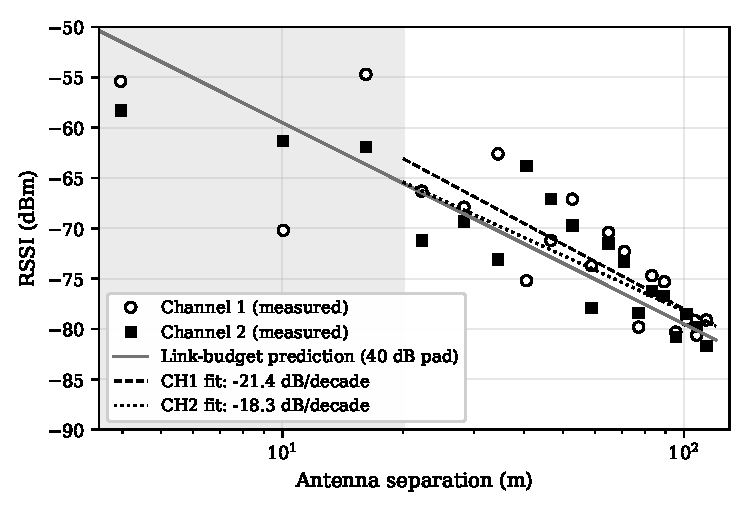
\includegraphics[width=0.48\textwidth]{figs/fig_rssi_vs_distance.pdf}
  \caption{Measured RSSI versus antenna separation for both receiver channels with a 40~dB
  attenuator in line, compared against the link-budget prediction. Fitted slopes of $-21.4$
  and $-18.3$~dB/decade are consistent with the $-20$~dB/decade free-space model; the shaded
  region below 20~m is excluded from the fit due to near-field and ground-proximity
  effects.}
  \label{fig:rssi}
\end{figure}

The scatter about the fits is not noise: residuals show 11--12~dB peak-to-peak
quasi-periodic ripple (Figure~\ref{fig:ripple}), consistent with two-ray ground-reflection
fading~\cite{rappaport2002}; at ${\approx}2$~m antenna heights the first Fresnel-zone
radius at midpath equals the antenna height. The channels also decorrelate: per-station
CH1$-$CH2 differences reach 11.4~dB with near-zero mean (Figure~\ref{fig:diversity}), so
the two antennas provide genuine spatial diversity, a small-scale instance of the
decorrelated fading that motivates best-source selection at range scale~\cite{bastie2022},
and the initial 120~m failure is explained as a fade-null-plus-boresight event rather than a
threshold crossing.

\begin{figure}[htbp]
  \begin{minipage}[t]{0.49\textwidth}
    \centering
    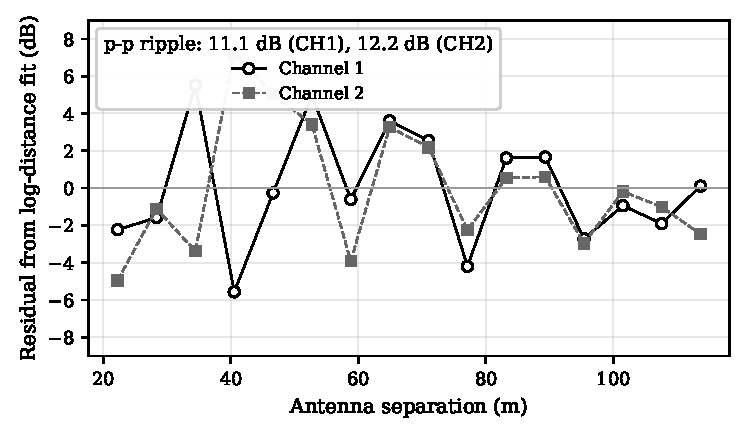
\includegraphics[width=\textwidth]{figs/fig_multipath_ripple.pdf}
    \caption{Residuals from the log-distance fit, showing 11--12~dB peak-to-peak ripple
    consistent with two-ray ground-reflection fading at the ${\approx}2$~m test antenna
    heights.}
    \label{fig:ripple}
  \end{minipage}\hfill
  \begin{minipage}[t]{0.49\textwidth}
    \centering
    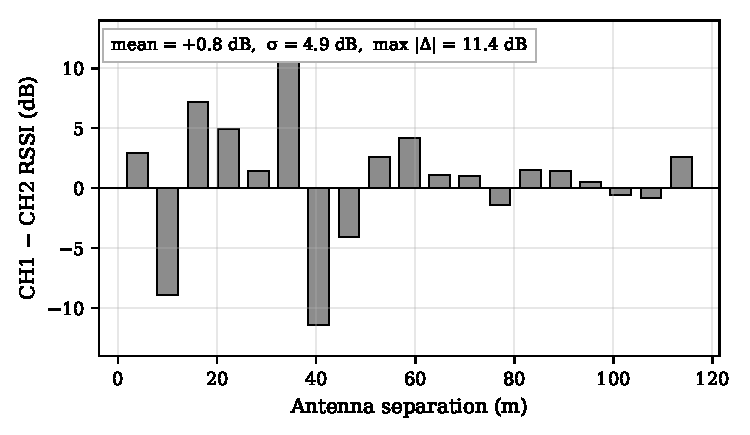
\includegraphics[width=\textwidth]{figs/fig_channel_diversity.pdf}
    \caption{Per-station RSSI difference between the two receive channels. Divergence up to
    11.4~dB with near-zero mean indicates decorrelated multipath fading across the two
    antennas, providing effective spatial diversity.}
    \label{fig:diversity}
  \end{minipage}
\end{figure}

Despite the fading, the $E_b/N_0$ readout held between 15.5 and 21~dB, BER was zero at every
sample, and the near-constant readout across 26~dB of RSSI change indicates the estimator
saturates near its ${\approx}20$~dB ceiling: the receiver never approached threshold.
Lock-loss counts showed no relationship to distance, implicating transient environmental
factors and possible front-end compression at high signal levels. The dataset therefore
bounds the margin from below: at EPL 120.6~dB the received power of $-80.6$~dBm sits
${\approx}15$~dB above the derived threshold and ${\approx}11$~dB above a conservative
threshold built on a 13~dB single-symbol $E_b/N_0$ requirement. The flight condition lies
2.6~dB beyond the farthest point tested; the characterization stands as a measured lower
bound with the derived $-95$~dBm estimate as the working threshold, and flight-specific
effects (Doppler, attitude nulls) justify retaining the onboard MEM/113 recording as
non-RF-dependent redundancy.

\subsection{End-to-End Channel Verification and Timing Integrity}\label{sec:res-chan}

\paragraph{Repetition rates and dropped frames.}
Sample timing was verified independently on both sides: transmit-side records show exactly
64.000~Hz (temperature) and 2048.00~Hz (pressure, \needsverify{see the commutation note in
\S\ref{sec:frame}}) with zero drops, and receive-side records reproduce the same rates,
confirming the frame structure of Section~\ref{sec:frame} from measurement. The ground logs
are not gap-free (temperature gaps to 156~ms and one 122-frame pressure gap), precisely
the event class the MEM/113 merge of \S\ref{sec:dropout} recovers.

\paragraph{Temperature channels at the ice point.}
Table~\ref{tab:temp} reports plateau statistics at the ice-point reference for the three
thermocouple channels on both sides of the link. Receive-side plateaus (8--13~s dwells)
show mean errors of $-0.26$ to $-0.07$~\si{\celsius} against the 0~\si{\celsius} reference
with standard deviations of 0.27--0.51~\si{\celsius}, against a measured quantization step
of 25~m\si{\celsius} (the TDC/102 least significant bit): the observed noise is genuine
channel noise of 10--20 counts, not resolution-limited. Transmit-side plateaus were
substantially shorter (0.8--1.8~s), had not fully equilibrated, and are reported as
indicative only.

\begin{table}[htbp]
  \centering
  \caption{Ice-point plateau statistics, temperature channels (\si{\celsius}).}
  \label{tab:temp}
  \begin{tabular}{llS[table-format=3.0]S[table-format=2.1]S[table-format=-1.3]S[table-format=1.3]}
    \toprule
    Side & Channel & {$n$} & {Dwell (s)} & {Mean} & {$\sigma$} \\
    \midrule
    RX (LDPS) & Temp4 & 593 & 9.3 & -0.157 & 0.350 \\
    RX (LDPS) & Temp5 & 829 & 12.9 & -0.262 & 0.269 \\
    RX (LDPS) & Temp13 & 522 & 8.1 & -0.072 & 0.513 \\
    TX (IADS, indicative) & temp4 & 49 & 0.8 & 0.578 & 0.747 \\
    TX (IADS, indicative) & temp5 & 112 & 1.7 & 0.368 & 0.246 \\
    TX (IADS, indicative) & temp13 & 113 & 1.8 & -0.207 & 0.566 \\
    \bottomrule
  \end{tabular}
\end{table}

The transmit-side capture additionally contains a synchronized anomalous excursion: exactly
83 samples above 500~\si{\celsius} on all three channels at once, two pinned at an identical
824.65~\si{\celsius}. The common-mode timing and identical clipped values indicate an
electrical or configuration artifact, not a thermal event. Two hypotheses are consistent
with the signature and will be separated before flight: a transient in the TDC/102
cold-junction or reference path, which would move all channels together by a common offset,
and an open-thermocouple detection pull-up asserting on all inputs, which would pin channels
at a rail-derived value. Shorting the inputs and repeating the capture distinguishes them.
These samples are excluded from Table~\ref{tab:temp}.

\paragraph{Pressure channels at static reference holds.}
Each pressure transducer was held at a steady tank pressure and captured on both sides
(Table~\ref{tab:pressure}). Transmit and receive statistics agree to 0.014~psi in mean and
to the third decimal in standard deviation: the RF and decommutation chain adds no
measurable bias or noise. Normalizing by full scale collapses all four channels to
${\approx}0.008$\%~FS, 4.9--5.4 ADC counts ($1\sigma$), a sensor-independent ADC/134 noise
floor. The 5000~psi transducer at 2\% of range retained 0.41~psi resolution, confirming
pad-monitoring utility before ignition. As discussed in \S\ref{sec:endtoend}, absolute
accuracy is bounded by the reference gauge (200~psi full scale, 10~psi graduations, no
marked class), which read ${\approx}100$~psi against the decommutated 100.28~psi for the
one hold recorded, within half-graduation readability; the other holds stand as precision
measurements.

\begin{table}[htbp]
  \centering
  \caption{Static-hold statistics, pressure channels (engineering units, psi).}
  \label{tab:pressure}
  \small
  \begin{tabular}{lS[table-format=3.3]S[table-format=1.3]S[table-format=3.3]S[table-format=1.3]S[table-format=1.4]S[table-format=1.1]}
    \toprule
    Sensor & {TX mean} & {TX $\sigma$} & {RX mean} & {RX $\sigma$} & {$\sigma$, \% FS} & {$\sigma$, counts} \\
    \midrule
    5000 psi & 100.278 & 0.415 & 100.265 & 0.413 & 0.0083 & 5.4 \\
    1000 psi & 73.686 & 0.083 & 73.683 & 0.083 & 0.0083 & 5.4 \\
    700 psi & 93.283 & 0.053 & 93.283 & 0.052 & 0.0076 & 4.9 \\
    350 psi & 91.749 & 0.028 & 91.749 & 0.028 & 0.0080 & 5.2 \\
    \bottomrule
  \end{tabular}
\end{table}

One metadata note: the LDPS export labeled the pressure values ``VDC'' while IADS presented
identical numbers as pressure, an ad hoc raw-data conversion during setup, retained as an
illustration of how readily semantic metadata diverges between tools once manual
conversions enter the chain (scenario~v of \S\ref{sec:fault}), and of a class of error that
only the configuration hash, which covers placement and width but not engineering-unit
labels, would \emph{not} catch; the staggered-stimulus procedure is its complement.

\subsection{Configuration-Skew Detection}\label{sec:res-fault}

The version-skew failure mode and its detection were demonstrated live, in the most
realistic direction: a configuration (XidML) omitting the counter was programmed into the
chassis while the ground retained its previous file pair, scenario~(i) with the skew
airborne. Throughout the 111~s stale-map period the receiver stayed locked and the SFID
cycled correctly (99.997\% of transitions), the silent regime, and the check word alone
exposed the mismatch: $\Delta = +1$ failed on the very first frame comparison
($\Delta = 13{,}422$), and over 80{,}171 subsequent comparisons the position formerly
carrying the counter passed by chance in only 0.59\% of isolated frames, never three
consecutively; a three-frame (1.5~ms) window yields zero false passes. The correct-pair
period passed 99.997\% of 74{,}863 comparisons, its two exceptions one $\Delta = 32$ event:
the odometer registering a 31-frame loss. Reprogramming the correct configuration restored
the staircase (Figure~\ref{fig:skew}).

\begin{figure}[htbp]
  \centering
  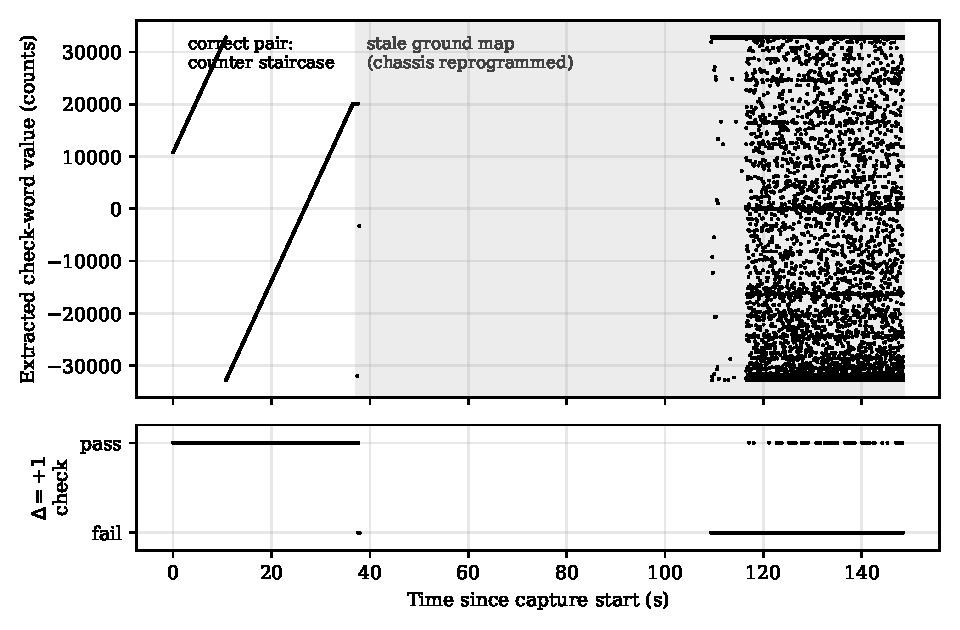
\includegraphics[width=0.5\textwidth]{figs/fig_skew_detect.pdf}
  \caption{Live configuration-skew detection. Extracted check-word value (top) and the
  $\Delta = +1$ test (bottom): the counter staircase under the correct file pair, and
  immediate, sustained check failure after a configuration omitting the counter was
  programmed into the chassis against the stale ground map (shaded). Receiver lock and
  SFID cycling remained intact throughout.}
  \label{fig:skew}
\end{figure}

\subsection{Reacquisition Statistics}\label{sec:res-reacq}

The interruption protocol was executed as 27 forced interruptions across 2--30~s nominal
dwells (0.5--30.7~s measured), both SMA feeds disconnected in each event, RSSI falling to
the channel noise floors; the ${\pm}0.5$~s channel-to-channel offsets reflect manual
handling of two connectors, so the bound below applies from signal restoration at each
input.

Three results follow: reacquisition is faster than the log resolves (all 27 events relocked
within the same 88.6~ms interval as RSSI restoration; channel~2 within $-1.5$ to $+0.6$~s
of channel~1); recovery is independent of outage duration from 0.5 to 30.7~s; and carrier
and bit-sync lock recovered together, the locked bit-sync count of
$3.2766$--$3.2782 \times 10^{6}$~counts/s independently confirming the bit rate.

Figure~\ref{fig:reacq} shows a representative 30~s event. Two limitations bound these
results: the test was conducted at an operating point (RSSI ${\approx}-79$ to $-81$~dBm,
$E_b/N_0 \approx 19$--20~dB) representative of the longest-path condition of the range
characterization (EPL ${\approx}120.6$~dB), i.e., near-flight signal levels but not near
threshold; and the 16-bit counter wraps every 32~s, longer than every outage tested here
but shorter than the flight, which is one reason the security channel of
\S\ref{sec:security} carries the counter's upper bits.

\paragraph{Transmitter power-cycle interruption.}
A transmitter power-cycle, additionally exercising start-up settling and cold-oscillator
reacquisition, was performed during a 137.2~s capture. The downlink lost 13.369~s (855
major frames, corroborated to 1.4\% by the retrieved-frame deficit), bounding the combined
off-dwell and reacquisition. Distinctly from the receive-side case, relock was followed by a
0.638~s transient dropping 41 major frames at alternating intervals before the stream
settled: lock declaration precedes clean data after a cold start.

\paragraph{Onboard-record continuity.}
The MEM/113 record spanning the event provides recoverability: packet sequence numbers
contiguous across the entire 1{,}035~s recording, all 428 packets covering the outage
present, and no sequence reset; the acquisition unit never power-cycled. Every sample the
downlink lost exists onboard. \needsverify{state whether the MEM/113 record is IRIG 106
Chapter~10 format with an embedded TMATS setup record; if so, note that this binds the
recording to its configuration (scenario~iii)}.

\paragraph{Content-aligned merge demonstration.}
\begin{sloppypar}
In the initial session the records differed by 1~d~05:01:26 (acquisition-unit clock versus
the LS-28 time module) and the parameter was recorded at 32~Hz against a 64~Hz downlink. A
repeat session resolved both: with the onboard stream re-logged at 64~Hz, a second
power-cycle (13.369~s, 854 frames, duration reproduced to the millisecond, the power-off
procedure itself) was captured with a deliberate thermal transient for identification.
Gap-aware time alignment identifies the downlinked parameter within the onboard record at
sample level: 99.60\% of 10{,}341 overlapping samples agree exactly (RMS 1.2 counts),
residuals confined to top-decile slew intervals (to 165~\si{\celsius}/s) where sub-frame
timing skew dominates. The onboard record supplies all 854 missing frames with clean
continuity at both edges (Figure~\ref{fig:merge}); onboard cadence measured 64.000~Hz
exactly with zero sequence breaks. The absolute offset, with ground time read as UTC, now
decomposes to exactly one day plus 1.1~s: the zone component resolved, leaving a date-field
error and ${\approx}1$~s set error before a fully timestamp-driven merge, which remains work
in progress. Disciplining the acquisition-unit clock from the TCG/105's GPS time, and
ultimately moving to Chapter~7 packet transport so that downlink and record share one
format, are the structural fixes.
\end{sloppypar}

\begin{figure}[htbp]
  \centering
  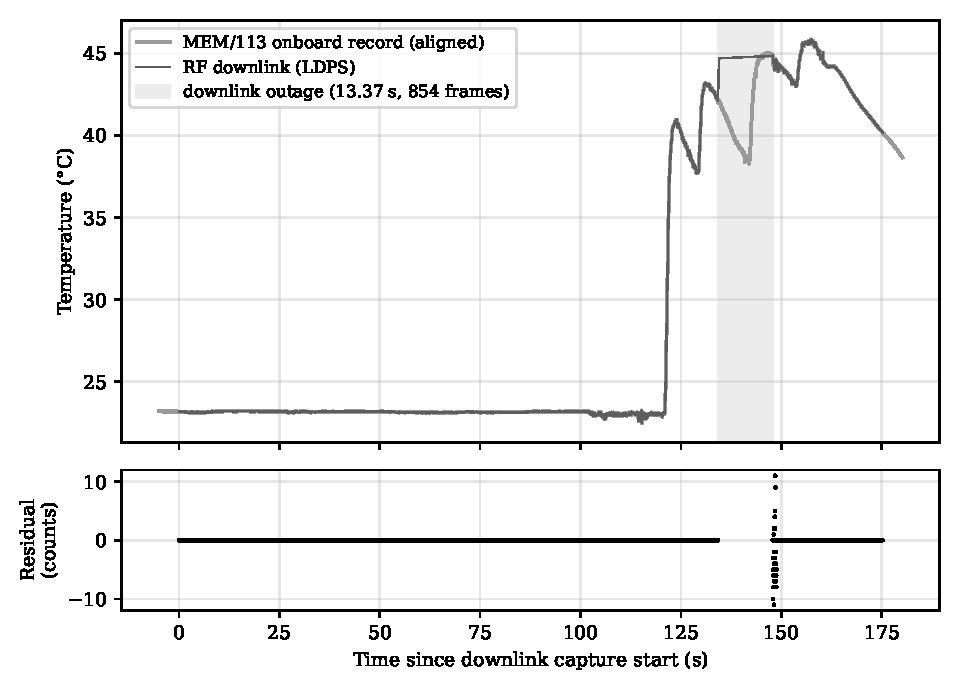
\includegraphics[width=0.5\textwidth]{figs/fig_merge_demo.pdf}
  \caption{Content-aligned merge demonstration. The onboard MEM/113 record (grey), aligned
  to the RF downlink (red) by gap-aware time alignment of raw counts, supplies all 854 frames
  lost during the 13.37~s transmitter power-cycle outage (shaded). Lower panel: per-sample
  residual between the records over the overlap; 99.60\% of samples agree exactly.}
  \label{fig:merge}
\end{figure}

\begin{figure}[htbp]
  \centering
  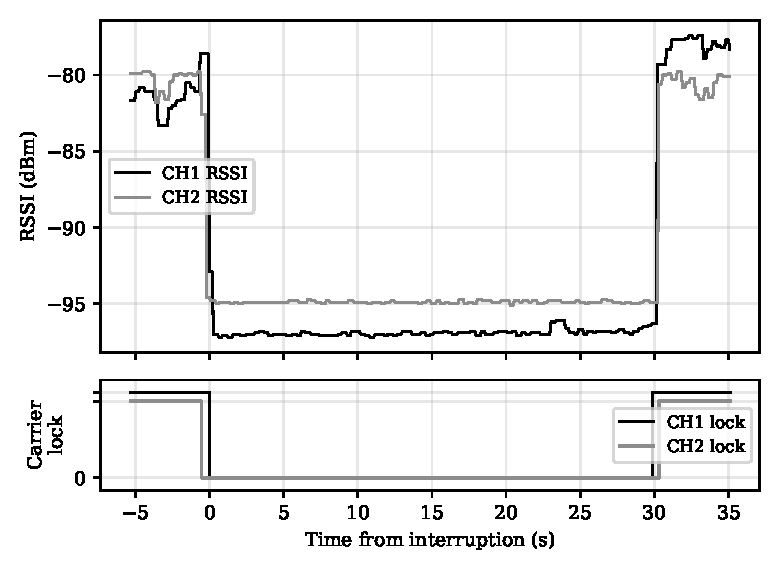
\includegraphics[width=0.48\textwidth]{figs/fig_reacq_event.pdf}
  \caption{Representative 30~s forced interruption: RSSI (top) and carrier lock (bottom)
  for both receiver channels. Lock returns within one 88.6~ms log interval of signal
  restoration.}
  \label{fig:reacq}
\end{figure}

\subsection{Stream Security: Software Demonstration}\label{sec:res-sec}

Table~\ref{tab:sec} summarizes the simulation of \S\ref{sec:security} on 10~s of the flight
frame (20{,}480 minor frames) with a 2~s dropout, 64 injected frames, one replayed major
frame, and bit-error rates of 0, $10^{-6}$ and $10^{-5}$, for profile~A with 64- and
32-bit tags and for profile~B; a 60~s run with a 34~s outage spanning a 16-bit counter wrap;
and two runs against a ground map skewed by one word, once with only the payload boundary
relocated (the geometry-preserving case of \S\ref{sec:fault}) and once with every security
word read from the wrong slot.

\begin{table}[htbp]
  \centering
  \caption{Security-layer simulation (\S\ref{sec:security}). Each run carries 64 injected frames (correct header, random payload) and one replayed major frame (32 frames). ``Delivered'' counts frames released to the user; ``non-genuine released'' those among them that are not bit-identical to the source (profile~B releases before authenticating and condemns 15.6~ms later). ``Lost beyond outage'' counts genuine frames after signal restoration that failed to decrypt. Transition density and longest run are for the serialized NRZ-L stream before and after the security layer.}
  \label{tab:sec}
  \scriptsize
  \begin{tabular}{@{}p{3.3cm}ccccccccc@{}}
    \toprule
    Profile & BER & Over- & Dropout & Delivered & Non-genuine & Rejected at & Lost beyond & Major frames & Cfg \\
            &     & head  & (s)     &           & released    & frame level & outage      & auth / fail / unverif. & hash \\
    \midrule
    A, 64-bit tag & 0 & 6\% & 2 & 16{,}384 & 0 & 96 (auth 64, replay 32) & 0 & -- & match \\
    A, 32-bit tag & 0 & 4\% & 2 & 16{,}384 & 0 & 96 (auth 64, replay 32) & 0 & -- & match \\
    B, deferred & 0 & 2\% & 2 & 16{,}448 & 64 & 32 (replay 32) & 0 & 506 / 4 / 3 & match \\
    A, 64-bit tag & $10^{-6}$ & 6\% & 2 & 16{,}355 & 0 & 125 (auth 93, replay 32) & 0 & -- & match \\
    A, 64-bit tag & $10^{-5}$ & 6\% & 2 & 16{,}131 & 0 & 348 (auth 316, replay 32) & 0 & -- & match \\
    B, deferred & $10^{-5}$ & 2\% & 2 & 16{,}447 & 313 & 32 (replay 32) & 0 & 304 / 202 / 8 & match \\
    A, 64-bit tag, 34~s outage across counter wrap & 0 & 6\% & 34 & 53{,}248 & 0 & 96 (auth 96, replay 0) & 0 & -- & match \\
    A, 64-bit tag, ground payload map relocated one word & 0 & 6\% & 2 & 0 & 0 & all (auth fail) & all & -- & mismatch \\
    A, 64-bit tag, ground reads security words from wrong slot & 0 & 6\% & 2 & 0 & 0 & all (no session) & all & -- & unreadable \\
    \bottomrule
  \end{tabular}

  \vspace{4pt}
  \begin{tabular}{@{}lcc@{}}
    \toprule
     & Plaintext stream & Secured stream \\
    \midrule
    NRZ-L transition density (per bit) & 0.378 & 0.491 \\
    Longest run without transition (bits) & 559 & 40 \\
    Frames with a bit error at BER $10^{-5}$ (profile A): flipped bits / frames failing authentication & \multicolumn{2}{c}{258 / 252} \\
    Software throughput, pure Python (ms per minor frame, encrypt / decrypt) & \multicolumn{2}{c}{0.44 / 0.46} \\
    \bottomrule
  \end{tabular}
\end{table}


Six observations follow. First, under profile~A every delivered frame is exact and every
injected and replayed frame is rejected, at both tag lengths; a forged frame that copies
the clear header and the security word verbatim still fails because the header is
associated data and the attacker has no key. Second, no genuine frame is lost beyond the
outage itself, at 2~s or at 34~s across the counter wrap: the first frame after signal
restoration decrypts. Third, under profile~B the 64 injected frames are released as pending
and condemned by the deferred tag of their major frame 15.6~ms later, the major frames
adjacent to the outage are reported incomplete or unverified, and replay is caught by the
counter; this is the cost of 2\% overhead stated as measured behavior rather than as a
caveat. Fourth, bit errors separate the profiles sharply. At $10^{-5}$ BER, roughly the
error rate at which PCM/FM is a few tenths of a decibel from its cliff, 258 flipped bits
cost profile~A the 252 frames that carried them (1.5\% of the frames received), which is
exactly the behavior wanted: a frame with an undetected bit error is a frame with a wrong
engineering value. The same 258 bits cost profile~B 202 of 514 major frames (39\%), because
one error anywhere condemns all 32 frames of its major frame, and 249 corrupted frames were
released to the user before the tag arrived. Per-frame authentication is therefore not only
the stronger property but the cheaper one in delivered data whenever the link is near
threshold. Fifth, the two skew cases fail differently and informatively. With only the
payload boundary relocated, the counter staircase is intact (the counter word is where the
ground expects it) and would by itself declare the stream consistent, the configuration
hash disagrees, and no frame authenticates: the hash and the tag catch what the counter
cannot. With every security word read from the wrong slot, the security channel never
parses, no session is established, and the counter never earns consistency: all three
witnesses fail. Sixth, encrypted payload words are uniformly distributed, so the serialized
stream's NRZ-L transition density rises from 0.38 to 0.49 transitions per bit and the
longest run falls from 559 bits (170~\si{\micro\second} of status-word zeros, enough to
stress a bit synchronizer) to about 40. For the payload, the cipher is also the randomizer,
and the clear words are too few to matter.

The configuration hash behaves as designed: relocating one parameter by one word changes
the 32-bit value; permuting the parameter list, or changing descriptions and
engineering-unit labels, does not. What the software does not demonstrate is the device
itself. Its timing closure at 3.2768~Mb/s, its frame synchronizer, the key-load procedure,
and the TMoIP re-emission path on the ground PC are the next build items and are reported
here as such.

\section{Lessons Learned}\label{sec:lessons}

\begin{itemize}
  \item COTS tooling relocates rather than removes integration risk: the failure-sensitive
  link is file consistency between the compiled frame definition and the exported parameter
  database, with no toolchain check of air-to-ground currency; budget verification effort
  there, not in the hardware. TMATS narrows the gap where both tools support it; it does
  not close it.
  \item Identify configurations by content, not by number. A configuration number is one
  more file to keep consistent; a hash of the frame map is computed independently by both
  sides and names the mismatch.
  \item A single frame word spent on a known counter converts the worst silent failure mode
  into a routine pre-flight check at 1\% of link capacity, and the same word is the nonce an
  authenticated cipher needs. Design the two together.
  \item A fixed attenuator is not a range simulator by itself; it multiplies the physical
  test separation ($10\times$ per 20~dB). Report pad value and separation together as
  equivalent path loss.
  \item At ground-test antenna heights the first Fresnel zone is obstructed: expect two-ray
  fading of 10~dB or more; a fixed-geometry pad sweep, not a walk-out, is the instrument for
  threshold measurement.
  \item Encryption is also a randomizer: payload transition density rose from 0.38 to 0.49
  and the longest run fell from 559 to about 40 bits.
  \item Keep recovery-critical functions (the Mx210 deployment altimeter) out of the
  telemetry chain entirely, and therefore out of reach of key management.
  \item Lock declaration is not clean data: after a transmitter power cycle, 41 major frames
  dropped over 0.64~s post-relock; validate the first second of post-relock data.
  \item Two undisciplined clocks cannot align two records (ours disagreed by 1~d~05:01:26):
  discipline both ends or align on content, record merge-critical parameters at the downlink
  rate, and consider Chapter~7 transport so that downlink and record share a format.
\end{itemize}

\section{Conclusion}

This paper set out from a claim about where the risk lives in a modern COTS telemetry
system: not in the hardware, but in the deployment gap between the configuration running in
the chassis and the file pair loaded on the ground. The staged campaign bore the claim out
at every layer: path-loss slopes of $-21.4$ and $-18.3$~dB/decade consistent with free
space, received power within 1--2~dB of budget, zero bit errors to 120.6~dB EPL, with the
measured 11.4~dB channel decorrelation motivating the orthogonally polarized diversity
configuration adopted for flight; ice-point mean errors of 0.26~\si{\celsius} or better and
a uniform ${\approx}5$-count (0.008\%~FS) pressure noise floor carried through the complete
chain; relock within one 88.6~ms log interval across 27 interruptions; and an onboard record
supplying all 854 frames lost to a 13.4~s transmitter outage, sample-exact against the
downlink.

The central demonstration closed the argument. A configuration omitting the check parameter
was programmed into the chassis against a stale ground map: the receiver stayed locked, the
SFID cycled, every parameter decommutated plausibly, and the frame-embedded counter failed
on the first frame, with zero measured false passes over 111~s under a three-frame window.
One sixteen-bit word, at 1.0\% of link capacity, converts the silent failure mode into a
pre-flight go/no-go check.

The paper then extended the argument in two steps that cost together between 2\% and 6\% of
the frame and nothing in the RF chain. A configuration hash turns detection into
identification and reaches the hand-edit class that no other check does. An
authenticated-encryption layer that reuses the counter as its nonce turns the ground
station's willingness to accept any plausible stream, the very property the skew
demonstration exposed, into a verified property: in software, every injected and replayed
frame was rejected, no frame was lost beyond the outages themselves, and the payload became
its own randomizer. What remains before flight is enumerable: the date-field correction
completing the timestamp-driven merge, automation of the verification tool, GPS-disciplined
operation, the remaining channels under the same verification pattern, and the encryptor
device and ground re-emission path. The broader conclusion travels beyond this vehicle: for
a program adopting COTS PCM telemetry, the architecture arrives correct by construction; the
engineering substance lies in verifying, identifying, and authenticating, continuously and
in the bitstream itself, that what the ground believes about the frame is what the vehicle
is actually transmitting.

\section{Acknowledgments}

The authors gratefully acknowledge Curtiss-Wright, NovAtel, Lumistar, and Haigh-Farr for
hardware and personnel support, and Quasonix for providing the program's transmitter;
Embry-Riddle Aeronautical University, Purdue University, and Virginia Tech for collaborative
assistance; and NASA MSFC, U.S. Army DEVCOM, Aerojet Rocketdyne, the Aerospace Corporation,
and the Morgan State University Administration, whose funding, initiative, and sustained
commitment made this program possible. Per ITC guidelines, the authors disclose the use of
Anthropic's Claude large language model in preparing this paper; the tool and extent of its
contribution are specified in~\cite{claude2026}.

{\footnotesize
\setlength{\bibsep}{0.5pt plus 0.5pt}
\bibliographystyle{unsrtnat}
\bibliography{references}}

\end{document}
